\documentclass[11pt]{article}
\usepackage[T1]{fontenc}

\usepackage[margin=1.05in]{geometry}
\usepackage{amsmath,amssymb,amsthm,mathtools}
\usepackage{microtype}
\usepackage{booktabs,tabularx,array}
\usepackage{enumitem}
\usepackage{xcolor}
\usepackage{tikz}
\usetikzlibrary{arrows.meta,positioning,calc}
\usepackage[hidelinks]{hyperref}
% \hypersetup{pdftitle={Report on Seymour's second-neighborhood proof},
%   pdfsubject={Mathathon Problem 58: historical context, proof map, motivation, and a blockwise proof}}
\newcommand{\abs}[1]{\lvert#1\rvert}
\newcommand{\ind}[1]{\mathbf 1_{\{#1\}}}
\newcommand{\Nplus}{N_1^+}
\newcommand{\Ntwo}{N_2^+}
\newcolumntype{Y}{>{\raggedright\arraybackslash}X}
\newtheorem{theorem}{Theorem}[section]
\newtheorem{lemma}[theorem]{Lemma}
% \theoremstyle{remark}
\newtheorem{remark}[theorem]{Remark}
\definecolor{ink}{HTML}{263B4E}
\definecolor{pale}{HTML}{F4F6F8}
\setlength{\emergencystretch}{2em}
\setlength{\parskip}{0.25em}
\setlist[itemize]{topsep=4pt,itemsep=2pt,leftmargin=1.6em}
\setlist[enumerate]{topsep=4pt,itemsep=3pt,leftmargin=1.8em}
\newcommand{\notespace}[2]{%
  \par\medskip\noindent\begin{minipage}{\linewidth}
  \textit{#1}\par\vspace{#2}\hrule height 0.3pt
  \end{minipage}\par\medskip}


\title{Report on Seymour's second-neighborhood proof}
\author{An Cao, Bernard Lidick\'y, Jan Volec}

\begin{document}
\maketitle
\vspace{-1.5em}

\begin{abstract}
Seymour's second-neighborhood conjecture, dated back to 1990, states
that every nonempty finite oriented graph has a vertex with at least as
many vertices at directed distance exactly two as at directed distance
one \cite{ghazal}. Recently, OpenAI released a manuscript claiming a
proof of this conjecture \cite{openai}. In this working report, we seek
to understand the argument and streamline parts of its presentation.
Our Mathathon work combines written
rewritings, proof diagrams, slides, and video animations as aids to
understanding. The contribution presented here is explanatory: we
reorganize existing arguments and identify directions for further
simplification and possible applications to related questions.
\end{abstract}

\section{Introduction and history of the problem}
\label{sec:intro}
\label{sec:history}

Seymour's conjecture asks for a local expansion phenomenon in a directed
graph: some vertex should reach at least as many new vertices in two
steps as it reaches in one step. Its apparent simplicity conceals a
basic difficulty. Different two-step paths can merge at the same
endpoint, and their endpoints may already be first neighbors. Counting
paths therefore does not directly count the distinct new vertices
required by the conjecture.

\subsection{The proposal and earlier approaches}
The conjecture is generally dated to 1990: Ghazal gives this date
explicitly \cite[p.~183]{ghazal}. Dean and Latka's 1995 paper is an
early published record \cite{deanlatka}, and is the source cited for
the conjecture in the OpenAI manuscript \cite[Section 1]{openai}.

The tournament case, often called Dean's conjecture, was proved by
Fisher in 1996 \cite{fisher}. Havet and Thomass\'e gave a short
constructive proof using median orders in 2000 \cite{havet}.
Tournaments have an arc between every pair of distinct vertices. The
general problem allows missing edges, so arguments exploiting that
completeness do not immediately cover all oriented graphs.

Two later developments are especially relevant to the proof studied
here. Brantner, Brockman, Kay, and Snively investigated minimal
counterexamples and graph-product constructions in their 2009 paper
\cite{bbks}. Seacrest developed an equivalent subset formulation in a
preprint first posted in 2018 and revised in 2019 \cite{seacrest}.
OpenAI explicitly builds on these approaches: its arc-deletion
argument adapts Seacrest's proof of Lemma 4, and the
transitive-tournament product already appears in Brantner et al.
\cite[Section 2]{openai}.

\subsection{Related conjectures}
Sullivan's 2006 survey records two related conjectures involving
\emph{in-neighbors}. One asks for a vertex with at least as many second
out-neighbors as first in-neighbors. The other compares the sum of the
first and second out-neighborhood sizes with twice the indegree
\cite[Conjectures 6.6 and 6.4]{sullivan}. We state these precisely in
Section~\ref{sec:ongoing}, where we discuss possible future applications.
The change from outdegree to indegree introduces an additional issue
that is not resolved by reversing the direction of every arc.

These questions also connect with short directed cycles. The
Caccetta--H\"aggkvist conjecture asks whether an $n$-vertex simple
digraph with minimum outdegree $r\ge1$ must have a directed cycle of
length at most $\lceil n/r\rceil$ \cite[Section 2]{sullivan}.
The OpenAI manuscript derives a directed-triangle consequence under
the stronger assumption that \emph{both} minimum indegree and minimum
outdegree are at least $n/3$ \cite[Corollary 6.1]{openai}.

\subsection{The recent OpenAI manuscript}
The manuscript \emph{A proof of Seymour's second-neighborhood
conjecture} is dated September 23, 2026 \cite{openai}, and was made
public in OpenAI's October 6, 2026 mathematics release \cite{release}.
It claims a proof for every nonempty finite oriented graph.
The argument passes through a minimal counterexample, a strengthened
inequality for subsets, a transitive-tournament blowup, and an
extremal contradiction using a pruning lemma.

Our report studies this argument as presented in the reviewed source.
Section~\ref{sec:reproof} gives a complete blockwise proof of its
blowup lemma under the stated subset-deficit hypothesis.
Section~\ref{sec:grid-pruning} explains the final extremal argument
assuming the source's pruning lemma, and describes the purpose of
the main constructions in the proof of that lemma. The matching and
rank bound itself remains a cited ingredient.

\subsection{Our work during the Mathathon}
Our project has focused on understanding and communicating the proof.
We traced the dependencies between the reductions and the final
contradiction, worked through the distinctions between ordinary images
and exact second neighborhoods, and rewrote the blowup calculation so
that its cancellation is visible one block at a time.

We also explored complementary ways to explain the argument: written
notes and alternative rewritings, presentation slides, static diagrams,
and animations or videos. The visual work is intended to make the
movement of vertices and grid points easier to follow, especially when
the proof changes from individual vertices to blocks and then to
families of ordered pairs. The working repository supplied by the team
is listed in the title block.

The project draws on the original manuscript together with explanations
and rewritings developed using OpenMath OS, Claude, Codex, and ChatGPT.
Comparing these presentations helped us identify places where a
definition, case distinction, or motivation needed to be made explicit.
The present report records the mathematical arguments in text; the
slides and animations provide supporting explanations. The assistance
and the limits of the verification claimed here are recorded at the end.

\section{Definitions and notations}
\label{sec:definitions}

An \emph{oriented graph} is a finite directed graph with no loops,
multiple arcs, or pair of opposite arcs. An \emph{arc} $u\to v$ is a
directed edge. 
For a vertex $v$, define its first and exact second out-neighborhoods by
\begin{align*}
 N_1^+(v)&=\{u:v\to u\},\\
 N_2^+(v)&=\{w\notin\{v\}\cup N_1^+(v):
                        v\to u\to w\text{ for some }u\}.
\end{align*}
Similarly, its first and exact second in-neighborhoods are
\begin{align*}
 N_1^-(v)&=\{u:u\to v\},\\
 N_2^-(v)&=\{w\notin\{v\}\cup N_1^-(v):
                        w\to u\to v\text{ for some }u\}.
\end{align*}
The word \emph{exact} means that a vertex already at distance one is
excluded from the distance-two neighborhood. Denote
\[
 d^+(v)=\abs{N_1^+(v)},\qquad d^-(v)=\abs{N_1^-(v)},\qquad
 d^{++}(v)=\abs{N_2^+(v)}.
\]
The \emph{converse} $D^{\mathrm{op}}$ is obtained by reversing every
arc of $D$.

A graph is \emph{strongly connected} if every vertex can reach every
other by a directed path. A \emph{tournament} has exactly one arc
between each pair of distinct vertices. It is \emph{transitive} if
the vertices admit an ordering in which every arc points forward.
We use $T_m$ for the transitive tournament on $[m]=\{1,\ldots,m\}$,
with $i\to j$ exactly when $i<j$.

For a graph $D$ and $A\subseteq V(D)$, define
\begin{equation}
 F_D(A)=\{y:x\to_D y\text{ for some }x\in A\},\qquad
 F_D^2(A)=F_D(F_D(A)).
 \label{eq:ordinary-image}
\end{equation}
These are ordinary images: $F_D(A)$ may meet $A$, and $F_D^2(A)$
may meet $F_D(A)$. Thus $F_D^2(A)$ is not an exact second
neighborhood. For a singleton in an oriented graph,
\[
 N_2^+(v)=F_D^2(\{v\})\setminus F_D(\{v\}),
\]
because there is no two-step return to $v$. We abbreviate $F_D$ to
$F$ when the graph is clear. 

\section{Problem statement and proof overview}
\label{sec:problem}

\subsection{The assertion and its in-neighborhood version}
The statement of the conjecture is as follows.

\begin{theorem}[Seymour's second-neighborhood assertion; {\cite[Theorem 1.1]{openai}}]
\label{thm:main}
Every nonempty finite oriented graph has a vertex $v$ satisfying
\[
                      \abs{N_1^+(v)}\le\abs{N_2^+(v)}.
\]
\end{theorem}

\begin{remark}
The corresponding assertion with $N_1^-(v)$ and $N_2^-(v)$ follows
from exactly the same statement. The converse $D^{\mathrm{op}}$ is an oriented graph, and for $k=1,2$,
\[
 N_k^+(v;D^{\mathrm{op}})=N_k^-(v;D).
\]
Applying Theorem~\ref{thm:main} to $D^{\mathrm{op}}$ therefore gives
a vertex $v$ satisfying
\[
                      \abs{N_1^-(v)}\le\abs{N_2^-(v)}.
\]
The inward and outward witnesses may be different. For the graph
consisting of a single arc $a\to b$, only $b$ satisfies the outward
inequality, and only $a$ satisfies the inward inequality. Reversal
changes both neighborhood directions; it does not give Sullivan's
mixed comparison between a second out-neighborhood and an indegree.
\end{remark}

The following sections present an overview of the proof in the source \cite{openai}.
\subsection{Two stages of extremal reasoning}
\label{sec:reduction-overview}
Assume that a counterexample exists. First choose one, $D$, with a
minimum number of vertices and, subject to that, a minimum number of
arcs. It has no sink. If it were not strongly connected, a strongly
connected component with no outgoing arc to another component would
give a smaller counterexample. Thus every vertex has positive
indegree. The source's arc-deletion argument then gives
\begin{equation}
 \abs{F_D^2(S)\setminus F_D(S)}<\abs{F_D(S)\setminus S}
       \qquad(\varnothing\ne S\subsetneq V(D)).
 \label{eq:subset-deficit}
\end{equation}
This is the source's Lemma 2.2. A transitive-tournament blowup converts
it into an oriented graph $G$ with positive indegrees and
\begin{equation}
 \abs U+\abs{F_G^2(U)}<2\abs{F_G(U)}
       \qquad(\varnothing\ne U\subsetneq V(G)),
 \label{eq:strict-concavity}
\end{equation}
as stated in its Lemma 2.3 and Proposition 2.1 \cite{openai}.

The second extremal choice takes place \emph{after $G$ is fixed}.
On the grid $V(G)\times V(G)$, choose two compatible families of
ordered pairs that maximize a score: their combined number of members
plus the number of points they leave uncovered. The subset inequality
produces larger candidate families. A pruning lemma removes their
conflicts at a sufficiently small cost that the resulting compatible
pair has a larger score, contradicting maximality. These are families
of ordered pairs, not merely two subsets of $V(G)$.

The graph minimization and the family maximization have different
purposes. The first forces the subset deficit. The second turns the
resulting strict subset inequality against itself. Section~\ref{sec:reproof}
reformulates the passage between them, and
Section~\ref{sec:grid-pruning} explains the final mechanism.

\subsection{Flowchart of the proof}
\label{sec:flow}

The left column constructs a graph with a strong subset inequality; the
right column shows why such a graph cannot exist. This is the conceptual route
through Sections 2--4 of the source \cite{openai}.

% \noindent\textbf{Families in the right column.}
% The grid consists of ordered pairs of vertices of $G$. A member of the
% first family covers points reached by moving its first coordinate along
% one directed edge; a member of the second covers points reached by
% moving its second coordinate. \emph{Compatible} means no point is
% covered by both families; \emph{uncovered} means covered by neither.
% The \emph{diagonal} consists of the pairs $(v,v)$. Family members are
% counted separately on each side.

\begingroup
\newcommand{\flowcell}[2]{%
  \begin{minipage}[t][2.3cm][t]{7cm}
  \raggedright\mbox{\textbf{#1}}\par\vspace{3pt}#2
  \end{minipage}}
\begin{center}
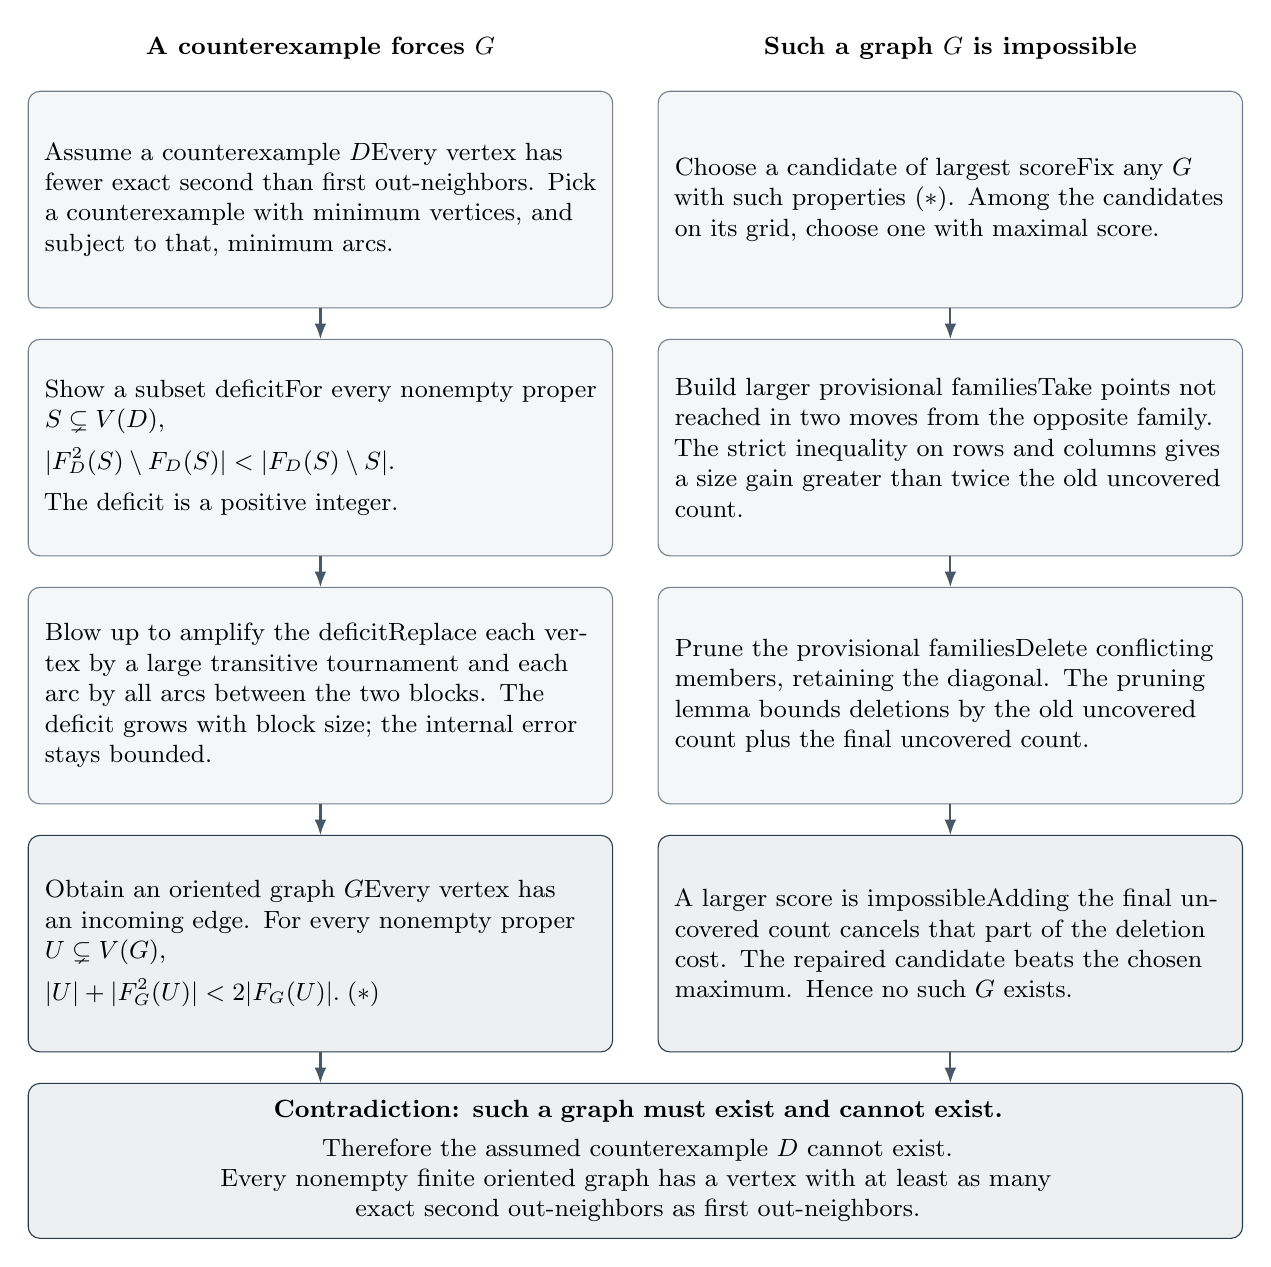
\begin{tikzpicture}[
 box/.style={draw=ink!65,fill=pale,rounded corners=1.5mm,
   text width=7cm,minimum height=2.75cm,align=left,
   inner sep=6pt,outer sep=0pt,font=\small},
 main/.style={box,draw=ink,fill=ink!8},
 arr/.style={-{Latex[length=2mm]},thick,draw=ink!85}
]
\node[align=center,font=\small\bfseries] at (-4,0.55)
 {A counterexample forces $G$};
\node[align=center,font=\small\bfseries] at (4,0.55)
 {Such a graph $G$ is impossible};

\node[box,anchor=north] (minimal) at (-4,0)
 {\flowcell{Assume a counterexample $D$}{%
 Every vertex has fewer exact second than first out-neighbors.
 Pick a counterexample with minimum vertices, and subject to that, minimum arcs.}};
\node[box,anchor=north] (optimal) at (4,0)
 {\flowcell{Choose a candidate of largest score}{%
 Fix any $G$ with such properties ($\ast$). Among the candidates
 on its grid, choose one with maximal score.}};

\node[box,anchor=north] (deficit) at (-4,-3.15)
 {\flowcell{Show a subset deficit}{%
 For every nonempty proper $S\subsetneq V(D)$,\\[4pt]
 $\abs{F_D^2(S)\setminus F_D(S)}
 <\abs{F_D(S)\setminus S}.$\\[4pt]
 The deficit is a positive integer.}};
\node[box,anchor=north] (candidates) at (4,-3.15)
 {\flowcell{Build larger provisional families}{%
 Take points not reached in two moves from the opposite family.
 The strict inequality on rows and columns gives a size gain greater
 than twice the old uncovered count.}};

\node[box,anchor=north] (blowup) at (-4,-6.3)
 {\flowcell{Blow up to amplify the deficit}{%
 Replace each vertex by a large transitive tournament and each arc by
 all arcs between the two blocks. The deficit grows with block size;
 the internal error stays bounded.}};
\node[box,anchor=north] (prune) at (4,-6.3)
 {\flowcell{Prune the provisional families}{%
 Delete conflicting members, retaining the diagonal. The pruning lemma
 bounds deletions by the old uncovered count plus the final uncovered
 count.}};

\node[main,anchor=north] (growth) at (-4,-9.45)
 {\flowcell{Obtain an oriented graph $G$}{%
 Every vertex has an incoming edge. For every nonempty proper
 $U\subsetneq V(G)$,\\[4pt]
 $\abs U+\abs{F_G^2(U)}<2\abs{F_G(U)}. \;(\ast)$}};
\node[main,anchor=north] (improvement) at (4,-9.45)
 {\flowcell{A larger score is impossible}{%
 Adding the final uncovered count cancels that part of the deletion
 cost. The repaired candidate beats the chosen maximum.
 Hence no such $G$ exists.}};

\node[main,anchor=north,text width=15cm,minimum height=0pt,align=center]
 (contradiction) at (0,-12.6)
 {\mbox{\textbf{Contradiction: such a graph must exist and cannot exist.}}\\[3pt]
 Therefore the assumed counterexample $D$ cannot exist.\\
 Every nonempty finite oriented graph has a vertex with at least as many\\
 exact second out-neighbors as first out-neighbors.};

\draw[arr] (minimal.south)--(deficit.north);
\draw[arr] (deficit.south)--(blowup.north);
\draw[arr] (blowup.south)--(growth.north);
\draw[arr] (optimal.south)--(candidates.north);
\draw[arr] (candidates.south)--(prune.north);
\draw[arr] (prune.south)--(improvement.north);
\draw[arr] (growth.south)--(contradiction.north -| growth.south);
\draw[arr] (improvement.south)--(contradiction.north -| improvement.south);
\end{tikzpicture}
\end{center}
\endgroup

\section{Blowup proof reformulation}
\label{sec:reproof}

\subsection{Why a blowup naturally amplifies the deficit}
\label{sec:motivation}
The reduction gives a difference between two boundary sizes, whereas
the final argument needs the three-term inequality
\eqref{eq:strict-concavity}. For any $S\subseteq V(D)$, let
\begin{equation}
 \delta(S)=\abs{F(S)\setminus S}-\abs{F^2(S)\setminus F(S)}.
 \label{eq:delta}
\end{equation}
For a nonempty proper $S$, the hypothesis is $\delta(S)\ge1$.
This suggests a natural amplification: replace each base
vertex by $m$ vertices so that each unit of this deficit contributes
an entire block of size $m$.

The connections between blocks make this work. Each base arc gives
all arcs from its source block to its target block. A single selected
vertex in an incoming block therefore fills the target block in the
first image. If $S$ records the blocks met by a chosen set $U$, the
base image $F(S)$ controls which full blocks appear.

There is still an internal error because $U$ may select only part of
a block. Transitive tournaments provide an order that bounds its
\emph{signed} contribution independently of $m$. If $f$ is the image
operator in $T_m$ and $T\ne\varnothing$ has smallest element $a$, then
\begin{equation}
 f(T)=\{a+1,\ldots,m\},\qquad
 T\setminus\{a\}\subseteq f(T),\qquad f^2(T)\subseteq f(T).
 \label{eq:tail-properties}
\end{equation}
Consequently $\abs T-2\abs{f(T)}+\abs{f^2(T)}\le1$.
The individual images may be large, but their signed contribution is
at most one. This separates the two scales: a deficit multiplied by
$m$, and an error bounded by the number $n$ of base vertices.

Our reformulation begins with a block's entire signed contribution,
\[
 c_v=\abs{U\cap B_v}-2\abs{F_G(U)\cap B_v}
                         +\abs{F_G^2(U)\cap B_v}.
\]
The proof below gives
\begin{equation}
 \abs U-2\abs{F_G(U)}+\abs{F_G^2(U)}
       \le -m\delta(S)+\abs{S\setminus F(S)}.
 \label{eq:budget}
\end{equation}
Thus $m>n$ makes the expression negative for proper support. Here
$n=\abs{V(D)}$, while the blowup has $nm$ vertices.

The source obtains this estimate by counting the first and second
images separately, introducing $F(S)\cup F^2(S)$, and enlarging an
internal-image sum. We collect the cancellation within each block
before summing. The construction, amplification principle, and sharper
intermediate error $\abs{S\setminus F(S)}$ are already present in
the original proof \cite[Lemma 2.3]{openai}; the reorganization makes
their roles more direct to check.

\subsection{Construction and statement}
Let $D$ be an oriented graph on $n\ge1$ vertices, and write $F=F_D$
as in \eqref{eq:ordinary-image}. Let $m$ be a positive integer. The
\emph{transitive-tournament blowup} $G=D[T_m]$ has vertex set
$V(D)\times[m]$ and blocks
\[
 B_v=\{(v,1),\ldots,(v,m)\}\qquad(v\in V(D)).
\]
Its arcs are precisely
\begin{equation}
 (u,i)\to_G(v,j)
 \quad\Longleftrightarrow\quad
 \bigl(u\ne v\text{ and }u\to_Dv\bigr)
 \ \text{or}\ 
 \bigl(u=v\text{ and }i<j\bigr).
 \label{eq:blowup-arcs}
\end{equation}
Call these arcs \emph{external} and \emph{internal}, respectively.
The ordinary out-image in $G$ is $F_G$, with $F_G^2=F_G\circ F_G$.
The internal image operator on labels is
\[
 f(T)=\{j\in[m]: i<j\text{ for some }i\in T\},
 \qquad f^2=f\circ f.
\]
For $A\subseteq[m]$, write $\iota_v(A)=\{(v,j):j\in A\}$; in
particular, $B_v=\iota_v([m])$. For any $U\subseteq V(G)$, set
\begin{equation}
 T_v=\{i\in[m]:(v,i)\in U\},\qquad
 S=\{v\in V(D):T_v\ne\varnothing\}.
 \label{eq:selection}
\end{equation}
Thus $U\cap B_v=\iota_v(T_v)$ and $S$ is its support in the base
graph. An indicator $\ind{\mathcal P}$ equals one when the condition
$\mathcal P$ holds and zero otherwise.

\begin{lemma}[Transitive-tournament blowup; reformulation of {\cite[Lemma 2.3]{openai}}]
\label{lem:blowup}
Suppose every vertex of $D$ has positive indegree and
\[
 \abs{F^2(A)\setminus F(A)}<\abs{F(A)\setminus A}
        \qquad(\varnothing\ne A\subsetneq V(D)).
\]
If $m>n$, then $G=D[T_m]$ is oriented, every vertex of $G$ has
positive indegree, and
\[
 \abs U-2\abs{F_G(U)}+\abs{F_G^2(U)}<0
        \qquad(\varnothing\ne U\subsetneq V(G)).
\]
\end{lemma}

\subsection{Proof by signed block contributions}
\begin{proof}
The graph $G$ is oriented by construction. A vertex in $B_v$ receives
an arc from every vertex in any block $B_u$ with $u\to_Dv$; such a
block exists because $v$ has positive indegree. Thus all indegrees in
$G$ are positive.

We first record the internal estimates. If $T\ne\varnothing$ and
$a=\min T$, then \eqref{eq:tail-properties} gives
$\abs T-\abs{f(T)}\le1$ and $f^2(T)\subseteq f(T)$. For
$T=\varnothing$ both images are empty. Therefore, for every
$T\subseteq[m]$,
\begin{equation}
 \begin{aligned}
 \abs T-2\abs{f(T)}&\le\ind{T\ne\varnothing},\\
 \abs T-2\abs{f(T)}+\abs{f^2(T)}&\le\ind{T\ne\varnothing}.
 \end{aligned}
 \label{eq:internal-bounds}
\end{equation}

Fix a nonempty proper set $U\subsetneq V(G)$ and use the notation
$T_v,S$ in \eqref{eq:selection}. The blocks partition $V(G)$, so
\begin{equation}
 \begin{aligned}
 \Phi(U)&:=\abs U-2\abs{F_G(U)}+\abs{F_G^2(U)}
           =\sum_{v\in V(D)}c_v,\\
 \text{where }c_v&:=\abs{T_v}-2\abs{F_G(U)\cap B_v}
                        +\abs{F_G^2(U)\cap B_v}.
 \end{aligned}
 \label{eq:proof-block-sum}
\end{equation}
We bound $c_v$ in two cases.

\medskip\noindent\textbf{Case 1: $v\in F(S)$.}
There is some $u\in S$ with $u\to_Dv$. Since $T_u$ is nonempty,
choose $i\in T_u$. Then $(u,i)\in U$, and for every $j\in[m]$ the
external arc $(u,i)\to_G(v,j)$ exists. Consequently
\[
 F_G(U)\cap B_v=B_v,
 \qquad\abs{F_G^2(U)\cap B_v}\le m.
\]
No exact description of the second intersection is needed for this bound.
Using $\abs{T_v}\le m$, and $T_v=\varnothing$ when $v\notin S$,
we obtain
\begin{equation}
 c_v\le\abs{T_v}-2m+m
       =\abs{T_v}-m
       \le -m\ind{v\notin S}.
 \label{eq:case-one}
\end{equation}

\medskip\noindent\textbf{Case 2: $v\notin F(S)$.}
We first identify the first image. If a vertex $(v,j)$ is reached in
one step from $U$ through an external arc, its predecessor lies in
some block $B_u$ with $u\in S$ and $u\to_Dv$. This would put
$v$ in $F(S)$, contrary to the case assumption. Thus the predecessor
must lie in $B_v$, and the internal arc condition says that
$i<j$ for some $i\in T_v$. Conversely, any such $i$ gives the
required internal arc from $U$. Hence
\begin{equation}
                    F_G(U)\cap B_v=\iota_v(f(T_v)).
 \label{eq:case-two-first}
\end{equation}

For the second image, a two-step walk with exactly one external arc
is impossible here. If the internal arc comes first, the external arc
runs from the starting block, which belongs to $S$, to $B_v$.
If the external arc comes first, the second, internal arc remains in
$B_v$, so the external arc again runs from a block in $S$ to $B_v$.
Either order would imply $v\in F(S)$.

If $v\in F^2(S)$, choose $u\in S$ and $w$ with
$u\to_Dw\to_Dv$, and choose $i\in T_u$. For every $j\in[m]$,
\[
                    (u,i)\to_G(w,1)\to_G(v,j)
\]
is a two-step walk using two external arcs. It reaches every vertex
of $B_v$, so $F_G^2(U)\cap B_v=B_v$. By
\eqref{eq:case-two-first} and the first estimate in
\eqref{eq:internal-bounds},
\[
                  c_v=\abs{T_v}-2\abs{f(T_v)}+m
                        \le m+\ind{v\in S}.
\]

If $v\notin F^2(S)$, two external arcs cannot reach $B_v$ from $U$:
their base vertices would exhibit $v\in F^2(S)$. The only remaining
walks have two internal arcs, whose endpoint labels are exactly
$f^2(T_v)$. Conversely, each such label is reached by those two
internal arcs. Thus $F_G^2(U)\cap B_v=\iota_v(f^2(T_v))$, and the
second estimate in \eqref{eq:internal-bounds} gives
\[
             c_v=\abs{T_v}-2\abs{f(T_v)}+\abs{f^2(T_v)}
                          \le\ind{v\in S}.
\]
The two alternatives combine to
\begin{equation}
 c_v\le m\ind{v\in F^2(S)}+\ind{v\in S}
                         \qquad(v\notin F(S)).
 \label{eq:case-two}
\end{equation}

From equations~\eqref{eq:case-one} and \eqref{eq:case-two}, we have
\begin{align}
 \Phi(U)=\sum_{v\in V(D)}c_v
 &\le -m\abs{F(S)\setminus S}
       +m\abs{F^2(S)\setminus F(S)}
       +\abs{S\setminus F(S)}\notag\\
 &=-m\delta(S)+\abs{S\setminus F(S)}.
 \label{eq:proof-budget}
\end{align}

If $\varnothing\ne S\subsetneq V(D)$, the hypothesis gives $\delta(S)\ge 1$. Since
$\abs{S\setminus F(S)}\le n$, we obtain
\[
                         \Phi(U)\le-m+n<0.
\]

It remains to handle $S=V(D)$, where the subset-deficit hypothesis does not
apply. Positive indegrees in $D$ give $F(S)=V(D)$.
Case 1 therefore fills every block, so $F_G(U)=V(G)$. Positive
indegrees in $G$ then give $F_G^2(U)=F_G(V(G))=V(G)$. Since $U$
is proper and $\abs{V(G)}=nm$,
\[
                  \Phi(U)=\abs U-2nm+nm=\abs U-nm<0.
\]
This proves the required inequality for every nonempty proper $U$.
\end{proof}


\clearpage
\section{Grids, pruning, and the extremal contradiction}
\label{sec:grid-pruning}

This section explains the motivation and application of the constructions
in Sections 3--4 of the original paper \cite{openai}. 

\section{Other relations: the Cooper--Mubayi paper}
\label{sec:other-relations}


\section{Proposed ongoing work}
\label{sec:ongoing}

\subsection{Making the pruning argument more intuitive}
We see an opportunity to ``humanize'' the proof ...

\subsection{Applications to related neighborhood questions}
Sullivan's two conjectures ask, respectively, for a vertex satisfying
\begin{align}
 d^{++}(v)&\ge d^-(v),\label{eq:sullivan-one}\\
 d^{++}(v)+d^+(v)&\ge2d^-(v).
 \label{eq:sullivan-two}
\end{align}
These appear as Conjectures 6.6 and 6.4 in Sullivan's survey
\cite{sullivan}. A basic obstacle to a direct transfer is
\begin{equation}
 d^{++}(v)-d^-(v)
 =\bigl(d^{++}(v)-d^+(v)\bigr)+\bigl(d^+(v)-d^-(v)\bigr).
 \label{eq:sullivan-obstruction}
\end{equation}
A Seymour vertex controls the first term, but need not control the
degree imbalance in the second. If the same vertex satisfies
$d^+(v)\ge d^-(v)$, it satisfies both Sullivan inequalities. In
particular, on graphs with indegree equal to outdegree at every
vertex, the vertex conditions coincide. This observation does not
provide the missing degree control in a general oriented graph.

We would like to identify a subset inequality incorporating both
incoming and outgoing information, and investigate which parts of
the grid and pruning argument could still be used. Potential tests
include the admissibility of the diagonal, the containment of opposite
corners in an old uncovered set, and a score that compensates the
resulting deletion cost. Any extension must verify these steps rather
than infer Sullivan's conclusions from the outward inequality alone.

\section*{AI Use Statement}
The mathematical starting point is the OpenAI manuscript
\cite{openai} and the earlier papers cited above. The blowup
construction, amplification idea, pruning lemma, and extremal
contradiction belong to those sources. Our contribution here is the
blockwise organization of the blowup proof and a guided exposition
of the surrounding argument.

We acknowledge ChatGPT, an OpenAI tool, for assistance in preparing
this report, including organization, drafting, clarification of
definitions, comparison of proof presentations, and algebraic and
set-theoretic cross-checks. GPT-6 Astra Pro assisted with the assembly
and revision of this report. The team's work also used OpenMath OS,
Claude, and Codex to develop alternative explanations, rewritings,
and supporting materials. The combination of the original paper,
these aids, and our discussions guided our understanding.

The assistance described here is not a claim of a new formal
verification. This report includes a complete elementary argument
for the stated blowup lemma and an explanation of the final
contradiction conditional on the cited pruning lemma. 

\begin{thebibliography}{10}

\bibitem{openai}
OpenAI.
\emph{A proof of Seymour's second-neighborhood conjecture}.
Preprint, September 23, 2026.

\bibitem{ghazal}
Salman Ghazal.
A remark on the second neighborhood problem.
\emph{Electronic Journal of Graph Theory and Applications}
\textbf{3}(2) (2015), 182--190.
\href{https://doi.org/10.5614/ejgta.2015.3.2.6}{doi:10.5614/ejgta.2015.3.2.6}.

\bibitem{deanlatka}
Nathaniel Dean and Brenda J. Latka.
Squaring the tournament---an open problem.
\emph{Congressus Numerantium} \textbf{109} (1995), 73--80.
Historical attribution follows \cite{openai}; bibliographic details
are also recorded in \cite{fisher}.

\bibitem{fisher}
David C. Fisher.
Squaring a tournament: A proof of Dean's conjecture.
\emph{Journal of Graph Theory} \textbf{23}(1) (1996), 43--48.
\href{https://doi.org/10.1002/(SICI)1097-0118(199609)23:1<43::AID-JGT4>3.0.CO;2-K}{Publisher DOI link}.

\bibitem{havet}
Fr\'ed\'eric Havet and St\'ephan Thomass\'e.
Median orders of tournaments: A tool for the second neighborhood
problem and Sumner's conjecture.
\emph{Journal of Graph Theory} \textbf{35}(4) (2000), 244--256.
\href{https://doi.org/10.1002/1097-0118(200012)35:4<244::AID-JGT2>3.0.CO;2-H}{Publisher DOI link}.

\bibitem{bbks}
James Brantner, Greg Brockman, Bill Kay, and Emma Snively.
Contributions to Seymour's second neighborhood conjecture.
\emph{Involve} \textbf{2}(4) (2009), 387--395.
Preprint: \href{https://arxiv.org/abs/0808.0946}{arXiv:0808.0946}.

\bibitem{seacrest}
Tyler Seacrest.
\emph{Seymour's second neighborhood conjecture for subsets of vertices}.
\href{https://arxiv.org/abs/1808.06293v3}{arXiv:1808.06293v3},
April 12, 2019; first posted August 20, 2018.

\bibitem{sullivan}
Blair D. Sullivan.
\emph{A summary of results and problems related to the
Caccetta--H\"aggkvist conjecture}.
\href{https://arxiv.org/abs/math/0605646}{arXiv:math/0605646},
submitted May 24, 2006. Especially Conjectures 6.4 and 6.6.
The year here follows the arXiv submission record.

\bibitem{release}
OpenAI.
\emph{Sharing AI progress in mathematics}.
October 6, 2026.
\href{https://openai.com/index/sharing-ai-progress-in-mathematics/}{Official release announcement}.

\end{thebibliography}
\end{document}